\documentclass[8pt]{beamer}

\usetheme[progressbar=frametitle]{metropolis}
\setbeamercolor{background canvas}{bg=white}

\usepackage{appendixnumberbeamer}

\usepackage{booktabs}
\usepackage[scale=2]{ccicons}

\usepackage{pgfplots}
\usepgfplotslibrary{dateplot}

\usepackage{xspace}
\newcommand{\themename}{\textbf{\textsc{metropolis}}\xspace}

\usepackage{lineno,hyperref}
\usepackage{amsmath}
\usepackage{mathtools}
\usepackage{amssymb}
\usepackage{xcolor}
\usepackage{pdfpages}
\usepackage{caption}
\usepackage{subcaption}
\usepackage{adjustbox}
\usepackage[document]{ragged2e}


\usepackage{amsbsy}
\newcommand*{\claps}[1]{\hbox to 0pt{\hss#1\hss}}
\newcommand*{\mat}[1]{\boldsymbol{\mathrm{#1}}}
\newcommand*{\subdims}[3]{\clap{\raisebox{#1}[0pt][0pt]{$\scriptstyle(#2 \times #3)$}}}
\fboxrule=1pt

\title{Supercritical Extraction}
\subtitle{A process model and a sensitivity analysis}
% \date{\today}
\date{11.06.2021}
\author{Oliwer Sliczniuk}
\institute{Aalto University}

\begin{document}
	
	\begin{frame}[fragile]{Model description}
		\large{\textbf{Supercritical Extraction: A process model and a sensitivity analysis}}\\
		\small{Oliwer Sliczniuk, Pekka Oinas, Francesco Corona} 
		\vfill
		\begin{minipage}{0.75\linewidth}
		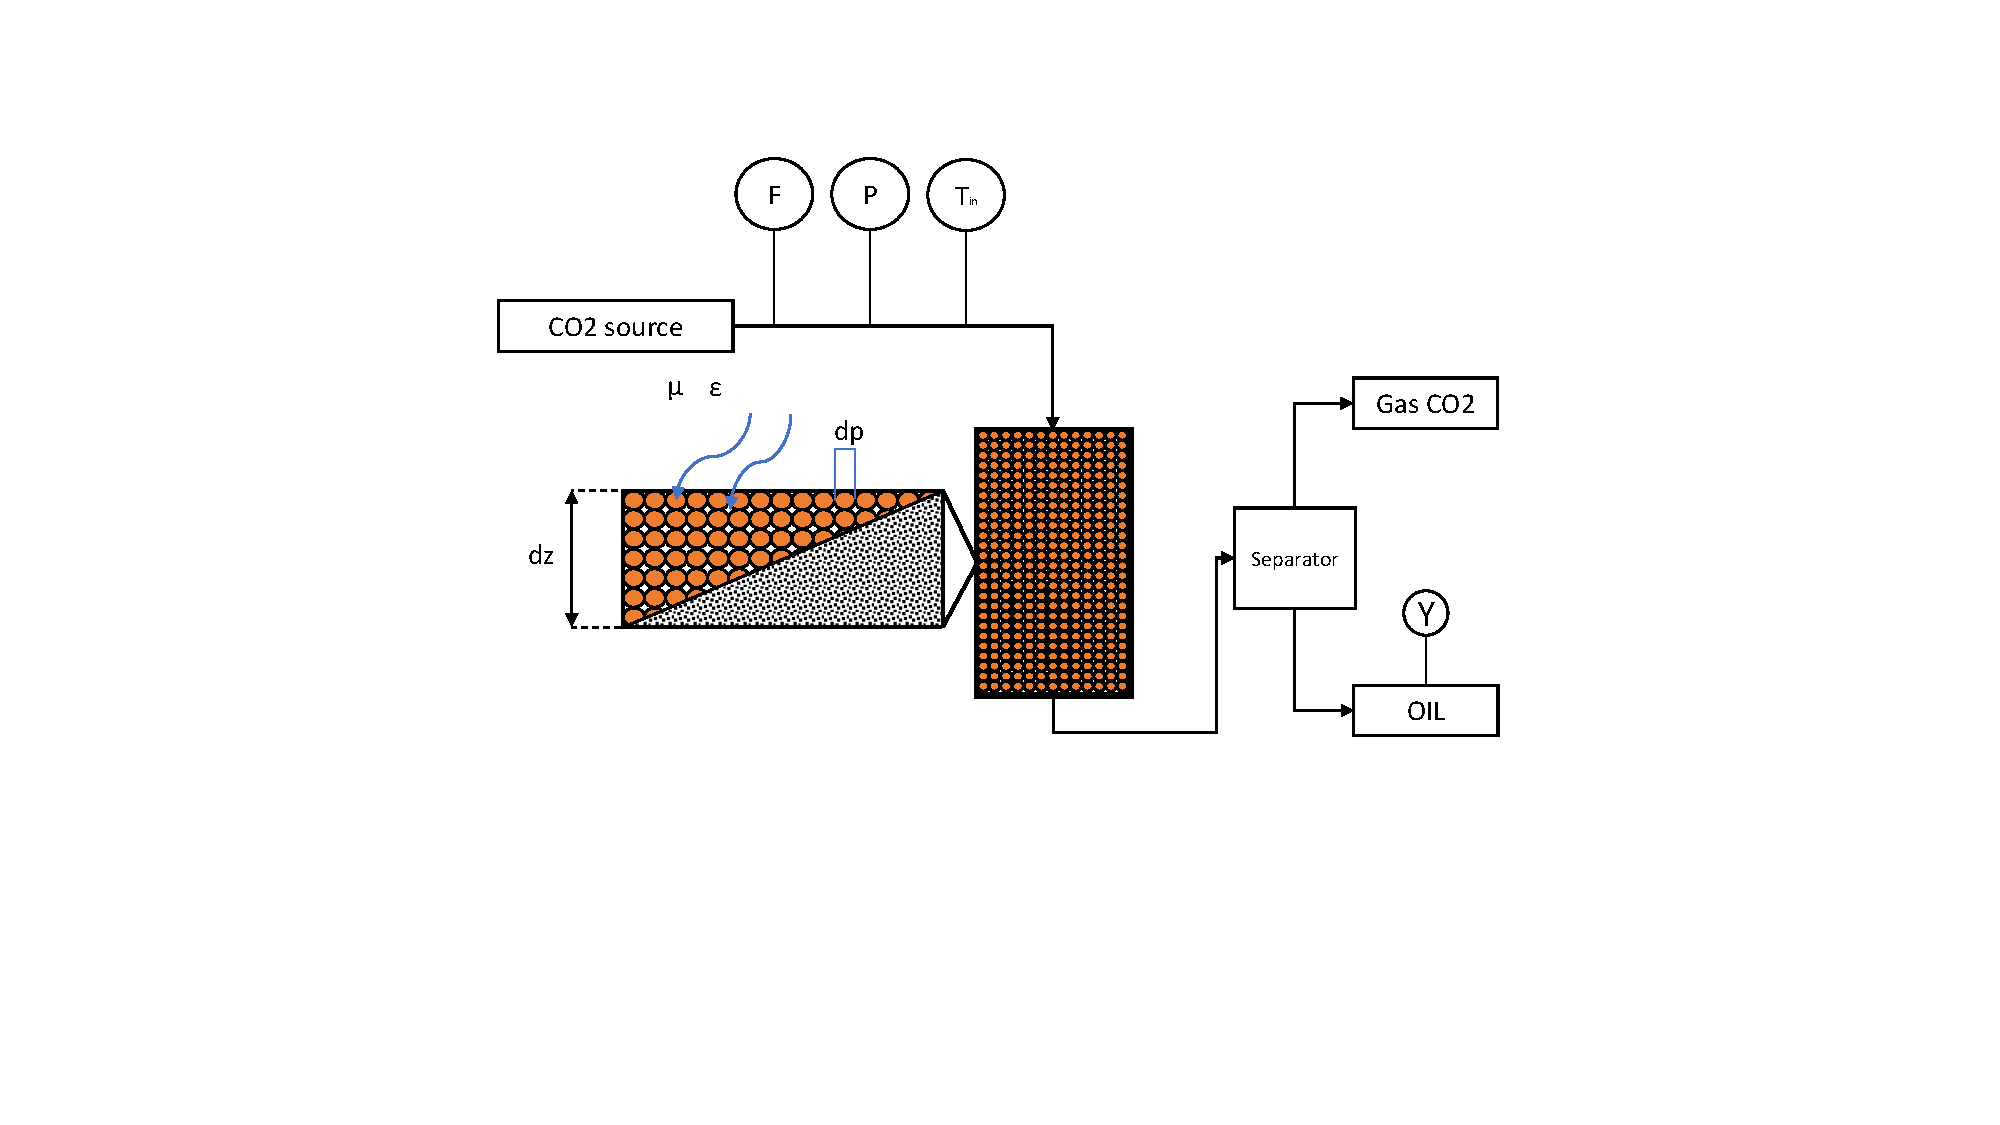
\includegraphics[trim = 6cm 5cm 6cm 2cm,clip,width=\linewidth]{Figures/SFE.pdf}
		\end{minipage}
		\begin{minipage}{0.24\linewidth}
			\begin{itemize}
				\item One-dimensional model
				\item Plug flow 
				\item No pressure drop
				\item Negligible external diffusion 
				\item Single component
				\item Pseudo-homogeneous thermal properties
				\item Uniformly distribution of the particles
			\end{itemize}
		\end{minipage}
	\\	
	\end{frame}

	\begin{frame}[fragile]{Differential model of the extractor$^1$}\justifying
	\textcolor{blue}{State variables},
	\textcolor{red}{control variables}, 
	\textcolor{magenta}{parameters}, 
	\textcolor{orange}{other variables} (\textcolor{blue}{state vars}, \textcolor{magenta}{parameters})\\
	{\footnotesize\begin{align*}
			\intertext{\textbf{Fluid phase mass balance}}
			\cfrac{\partial \textcolor{blue}{c}(t,z)}{\partial t} &=  \underbrace{-\cfrac{1}{ \textcolor{magenta}{\epsilon A}}\cfrac{\textcolor{red}{F}(t)}{\textcolor{orange}{\rho}(\textcolor{blue}{T}(t,z)\textcolor{red}{P}(t))} \cfrac{\partial \textcolor{blue}{c}(t,z)}{\partial  \textcolor{blue}{z}}}_{\text{Convection}}
			+ \underbrace{ \textcolor{orange}{D^M_e}(\textcolor{blue}{T}(t,z)\textcolor{red}{P}(t)) \cfrac{\partial^2 \textcolor{blue}{c}(t,z)}{\partial \textcolor{blue}{z^2}} }_{\text{Diffusion}}
			+ \underbrace{ \cfrac{1-\textcolor{magenta}{\epsilon}}{\textcolor{magenta}{\epsilon}} \textcolor{blue}{r_e}(t,z) }_{\text{Kinetics}}\\
			%		\end{align*}}
			\intertext{\textbf{Solid phase mass balance}}
			%		{\scriptsize\begin{align*}
			\cfrac{\partial \textcolor{blue}{q}(t,z)}{\partial t} &= \underbrace{ \textcolor{blue}{r_e}(t,z) }_{\text{Kinetics}}\\
			%		\end{align*}}
			\intertext{\textbf{Heat balance}}
			%		{\scriptsize\begin{align*}
			\cfrac{\partial \textcolor{blue}{T}(t,z)}{\partial t} &= 
			\underbrace{ -\cfrac{\textcolor{red}{F}(t)}{\textcolor{magenta}{A}} \cfrac{\textcolor{orange}{C_p}(\textcolor{blue}{T}(t,z)\textcolor{red}{P}(t))}{ [(1-\textcolor{magenta}{\epsilon})\textcolor{orange}{\rho}(\textcolor{blue}{T}(t,z)\textcolor{red}{P}(t)) \textcolor{orange}{C_p} (\textcolor{blue}{T}(t,z)\textcolor{red}{P}(t)) + \textcolor{magenta}{ \epsilon \rho_s C_{ps} } ]} \cfrac{\partial \textcolor{blue}{T}(t,z)}{\partial \textcolor{blue}{z}}  }_{\text{Convection}}
			+ \underbrace{ \textcolor{orange}{D^T_e}(\textcolor{blue}{T}(t,z)\textcolor{red}{P}(t)) \cfrac{\partial^2 \textcolor{blue}{T}(t,z)}{\partial \textcolor{blue}{z^2}} }_{\text{Diffusion}}\\ \\
			%		\end{align*}}
			\intertext{Extraction kinetics}
			%		{\scriptsize\begin{align*}
			\textcolor{blue}{r_e}(t,z) &= -\cfrac{\textcolor{orange}{D_i}(\textcolor{blue}{T}(t,z))}{\textcolor{magenta}{ \mu l^2} }\left(\textcolor{blue}{q}(t,z) - \textcolor{blue}{c}(t,z) \cfrac{\textcolor{magenta}{\rho_s}}{\textcolor{orange}{k_m}(\textcolor{blue}{T}(t,z))\textcolor{orange}{\rho}(\textcolor{blue}{T}(t,z)\textcolor{red}{P}(t))} \right)
			%		\end{align*}}
			\\ \\
			\hline 
			\textbf{Measurment - Yield}\\
			%		{\scriptsize\begin{align*}
			y(t) &= \cfrac{\sum\limits_{i=1}^{N_z}  \left(  \textcolor{magenta}{\cfrac{1}{N_z}} \left(\textcolor{magenta}{m_0} - m_i(\textcolor{blue}{q_i}(t,z)) \right) \right) }{\textcolor{magenta}{m_0}} = \underbrace{ \cfrac{\sum\limits_{i=1}^{N_z}  \left(  \textcolor{magenta}{\cfrac{V}{N_z}} \left(\textcolor{magenta}{q_0} - \textcolor{blue}{q}_i(t,z) \right) \right) }{\textcolor{magenta}{q_0 V}} }_{g(x(t))}
	\end{align*}}
	\hrule
	\footnotesize{[1] E. Reverchon, Mathematical modeling of supercritical extraction of sage oil, AIChE J 42 (6), 1996}
	\end{frame}

	\begin{frame}[fragile]{PDE to ODE and sensitivity analysis}\justifying
		Sensitivity analysis$^2$ measures the susceptibility of the model to changes in its parameters\\
		\footnotesize{
			\begin{columns}[c]
				\column{.4\textwidth}
			\begin{align*}
				\cfrac{d x(t)}{d t} &= 
				\begin{bmatrix}
					\cfrac{d c_1(t)}{d t} 	  \\
					\vdots					  \\
					\cfrac{d c_{N_z}(t)}{d t} \\
					\\ \hline \\
					\cfrac{d q_1(t)}{d t} 	  \\
					\vdots					  \\
					\cfrac{d q_{N_z}(t)}{d t} \\
					\\ \hline \\
					\cfrac{d T_1(t)}{d t} 	  \\
					\vdots 					  \\
					\cfrac{d T_{N_z}(t)}{d t}
				\end{bmatrix}
				=
				\underbrace{\begin{bmatrix}
					F_1 \left( c(t),q(t),T(t); p \right)\\ 
					\vdots\\ 
					F_{N_z} \left( c(t),q(t),T(t); p \right)\\ \\
					\\ \hline \\ \\
					F_{N_z+1} \left( c(t),q(t),T(t); p \right)\\
					\vdots\\
					F_{2N_z} \left( c(t),q(t),T(t); p \right)\\ \\
					\\ \hline \\ \\
					F_{2N_z+1} \left( c(t),q(t),T(t); p \right) \\
					\vdots\\
					F_{3N_z} \left( c(t),q(t),T(t); p \right)
				\end{bmatrix}}_{F \left( t; p \right)} \\ 
			%Z &= \cfrac{\partial \textcolor{blue}{x}(t,p)}{\partial \textcolor{magenta}{p}} \nonumber \\
			\end{align*}
			\column{.4\textwidth}
			State sensitivity
			\begin{align*}
			\dot{Z}  & = \partial_t \textcolor{blue}{Z}(t,p) = \partial_t \left( \partial_p \textcolor{blue}{x}(t,p) \right) = \\
			& = \partial_p \left( \partial_t \textcolor{blue}{x}(t,p) \right) = \partial_p \textcolor{blue}{F}(x(t);p) \\
			\partial_p \textcolor{blue}{F}(x(t);p) &=  \underbrace{ \partial_{x(t)} F(x(t);p)}_{J_x(x(t);p)}  \underbrace{\partial_p x(t)}_{S(x(t);p)} + \underbrace{ \partial_p F(x(t);p) }_{J_p(x(t);p)}
		\end{align*}
		\\
		\vspace{0.1cm}
		\hrule
		\vspace{0.1cm}
		Output sensitivity \\
		\begin{align*}
			\cfrac{d y(t)}{dp} &= \cfrac{d g(x(t))}{dp} = \partial_{x(t)} g(x(t)) \; S(x(t);p)
		\end{align*}	
	\end{columns}
}
\hrule
\footnotesize{[2] T. Maly, L. R. Petzold, Numerical methods and software for sensitivity analysis of differential-algebraic systems, Applied Numerical Mathematics 20 (1-2), 1996 }
	\end{frame}
	
	\begin{frame}[fragile]{Sensitivity analysis - flow rate}
	\begin{table}[!hbt]
		\centering
		\begin{tabular}{ |c|c|c|c|c|c|c|c|c| } 
		\hline
		Ref& $F[kg/hr]$ & $T_{Inlet} [C]$ & $T_{extractor} [C]$ & $P [bar]$ & $c [kg/m^3]$ & $q [kg/m^3]$ \\ \hline
		Vargas$^3$ & 0.035      & 50              & 50		             & 90  	     & 0 		    & 27 		   \\ \hline
		\end{tabular}
	\end{table}				
	\begin{columns}[t]
		\column{.3\textwidth}
		\centering
		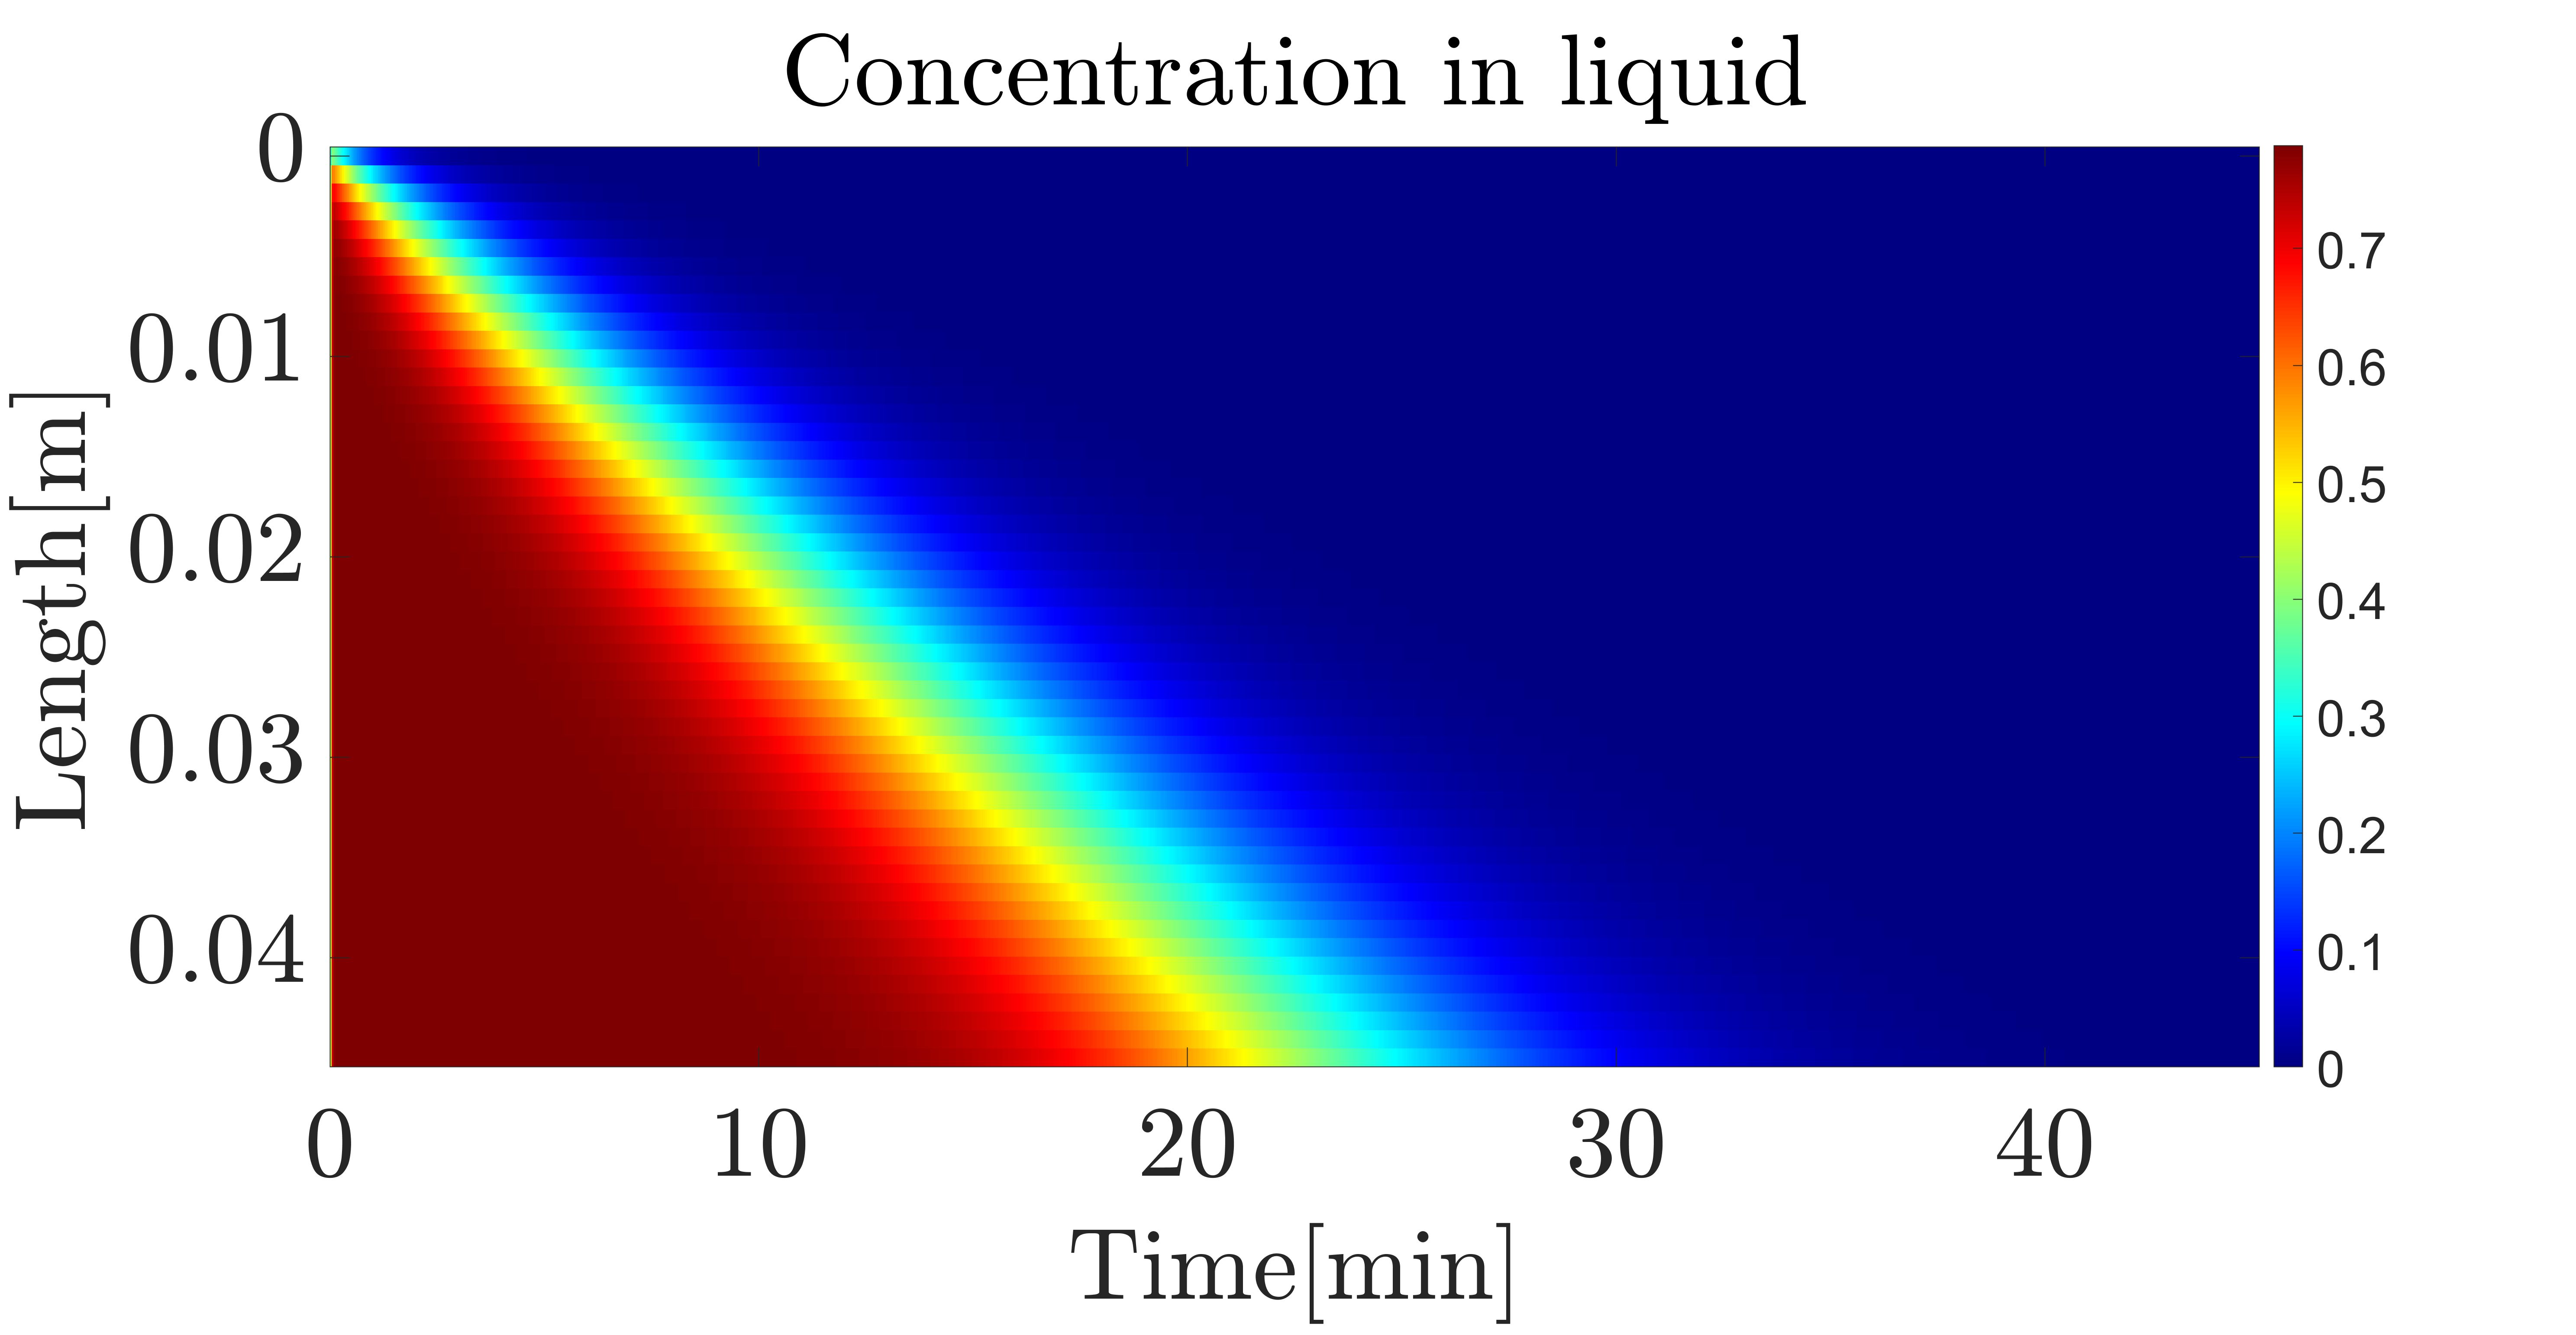
\includegraphics[width=3.7cm,height=2.0cm]{Figures/Sensitivity/ConcentrationLiquid.png}\\
		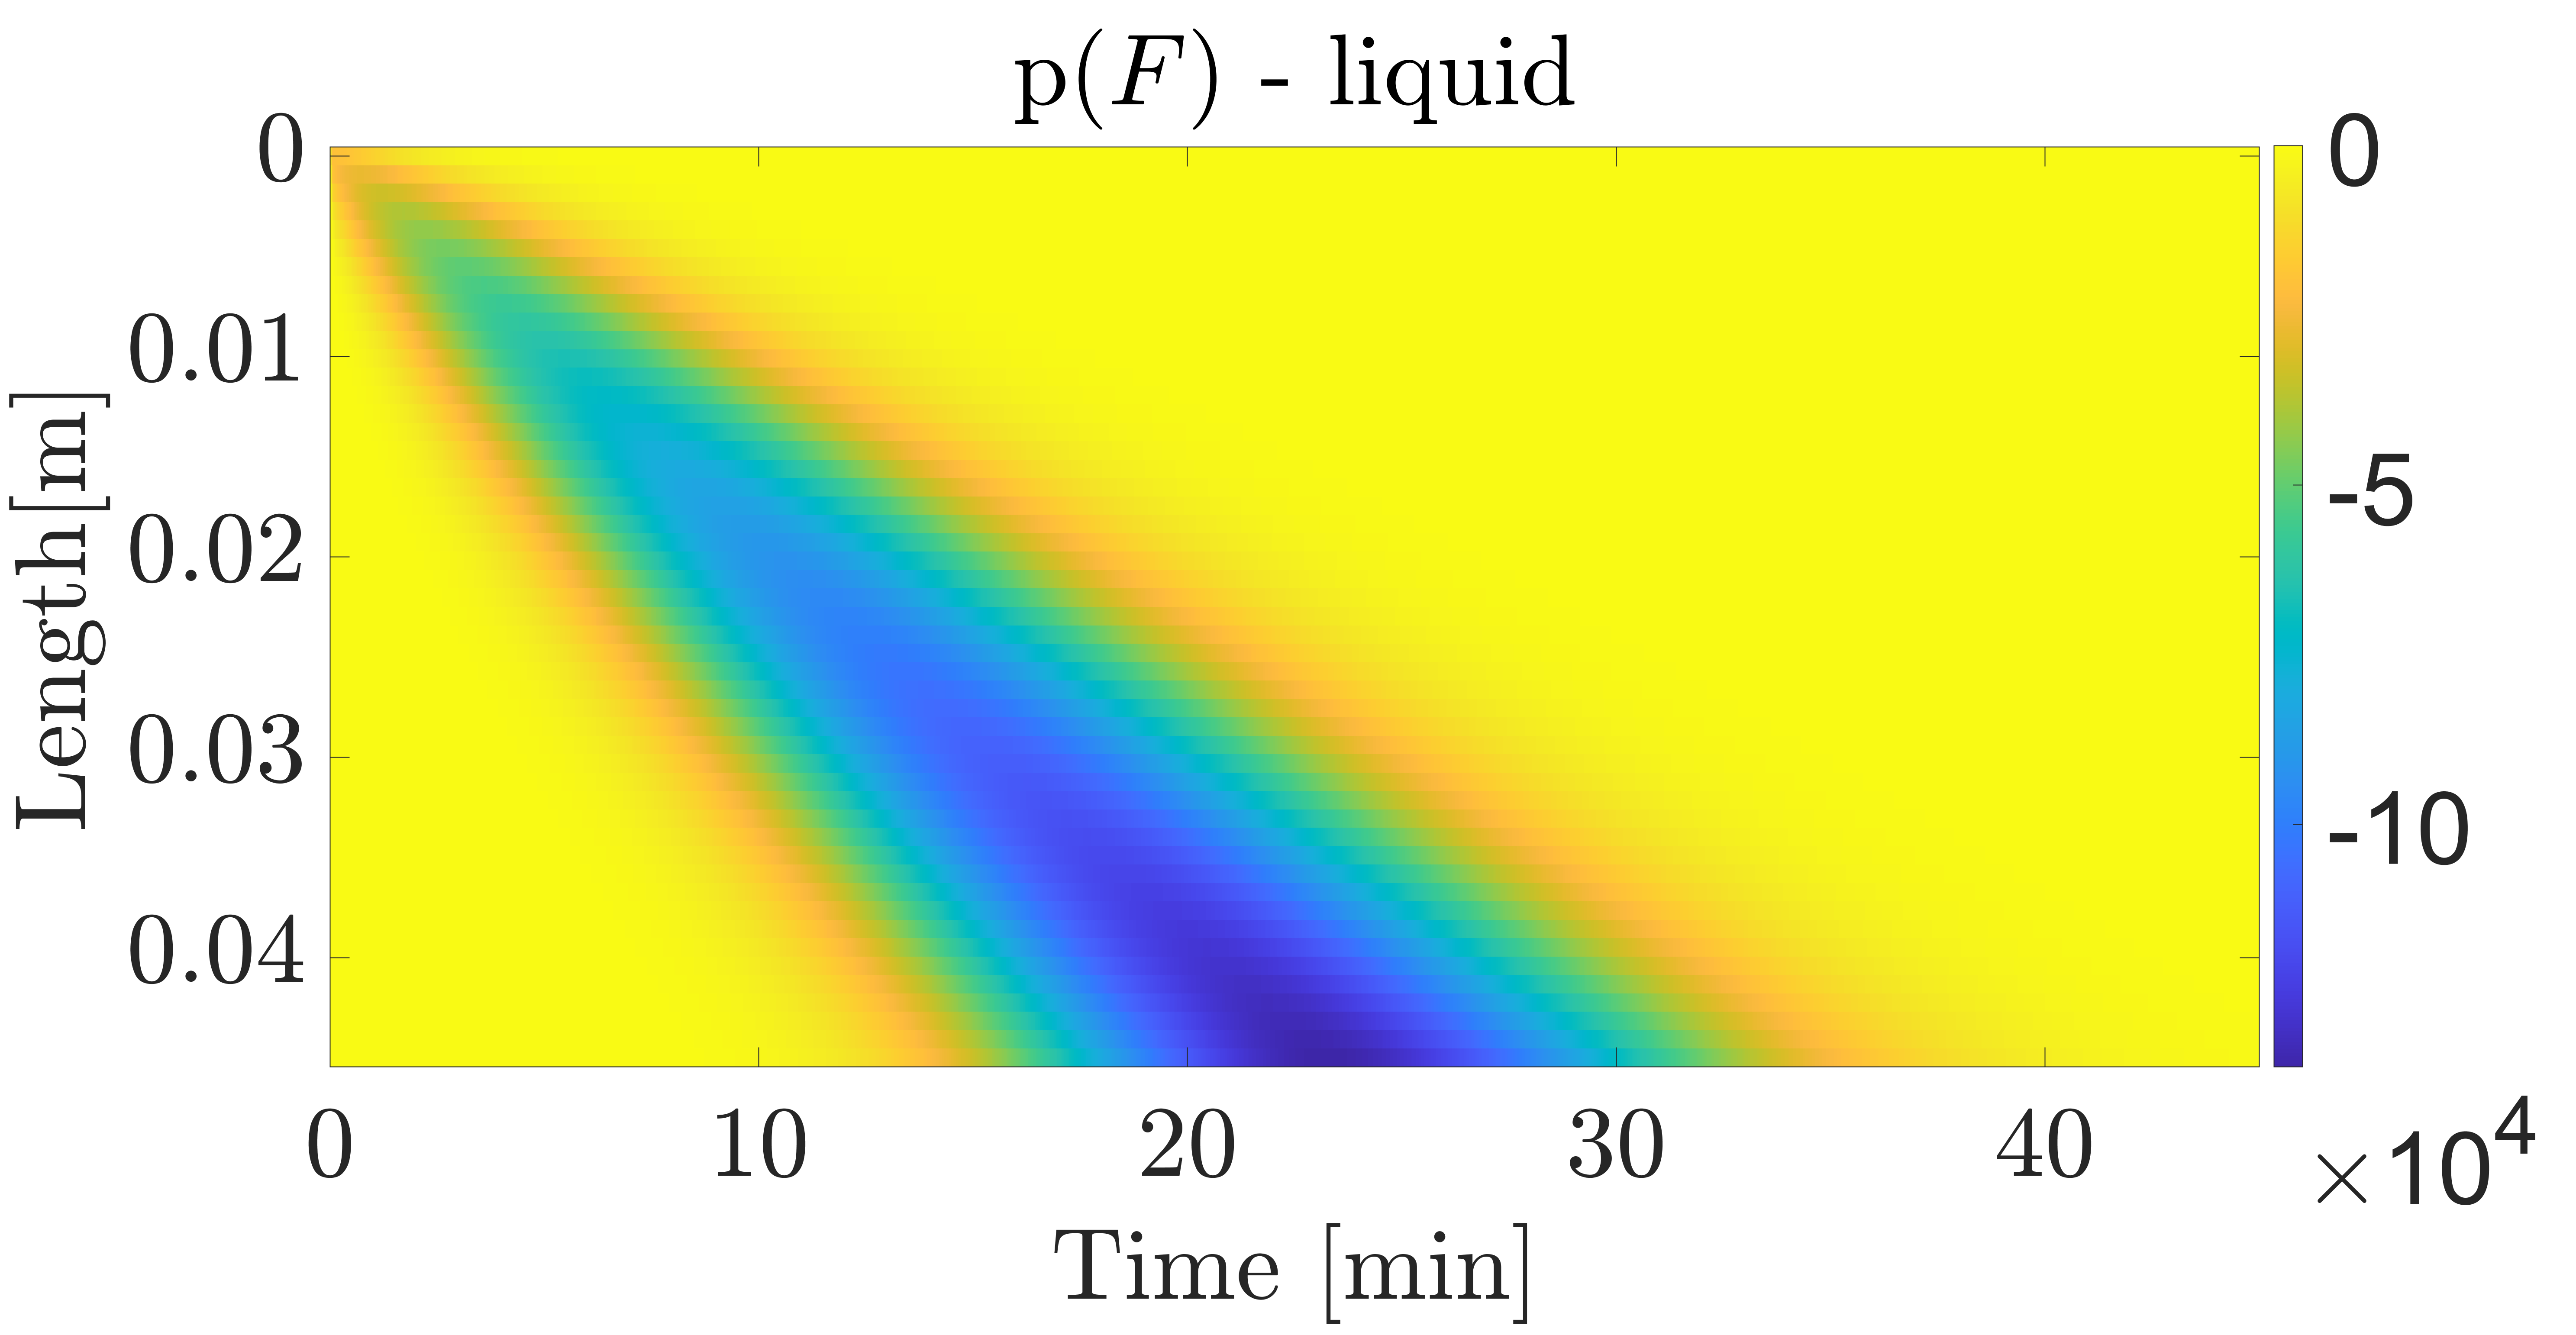
\includegraphics[width=3.7cm,height=2.0cm]{Figures/Sensitivity/Imagesc/2_SS_R_F.png}\\
		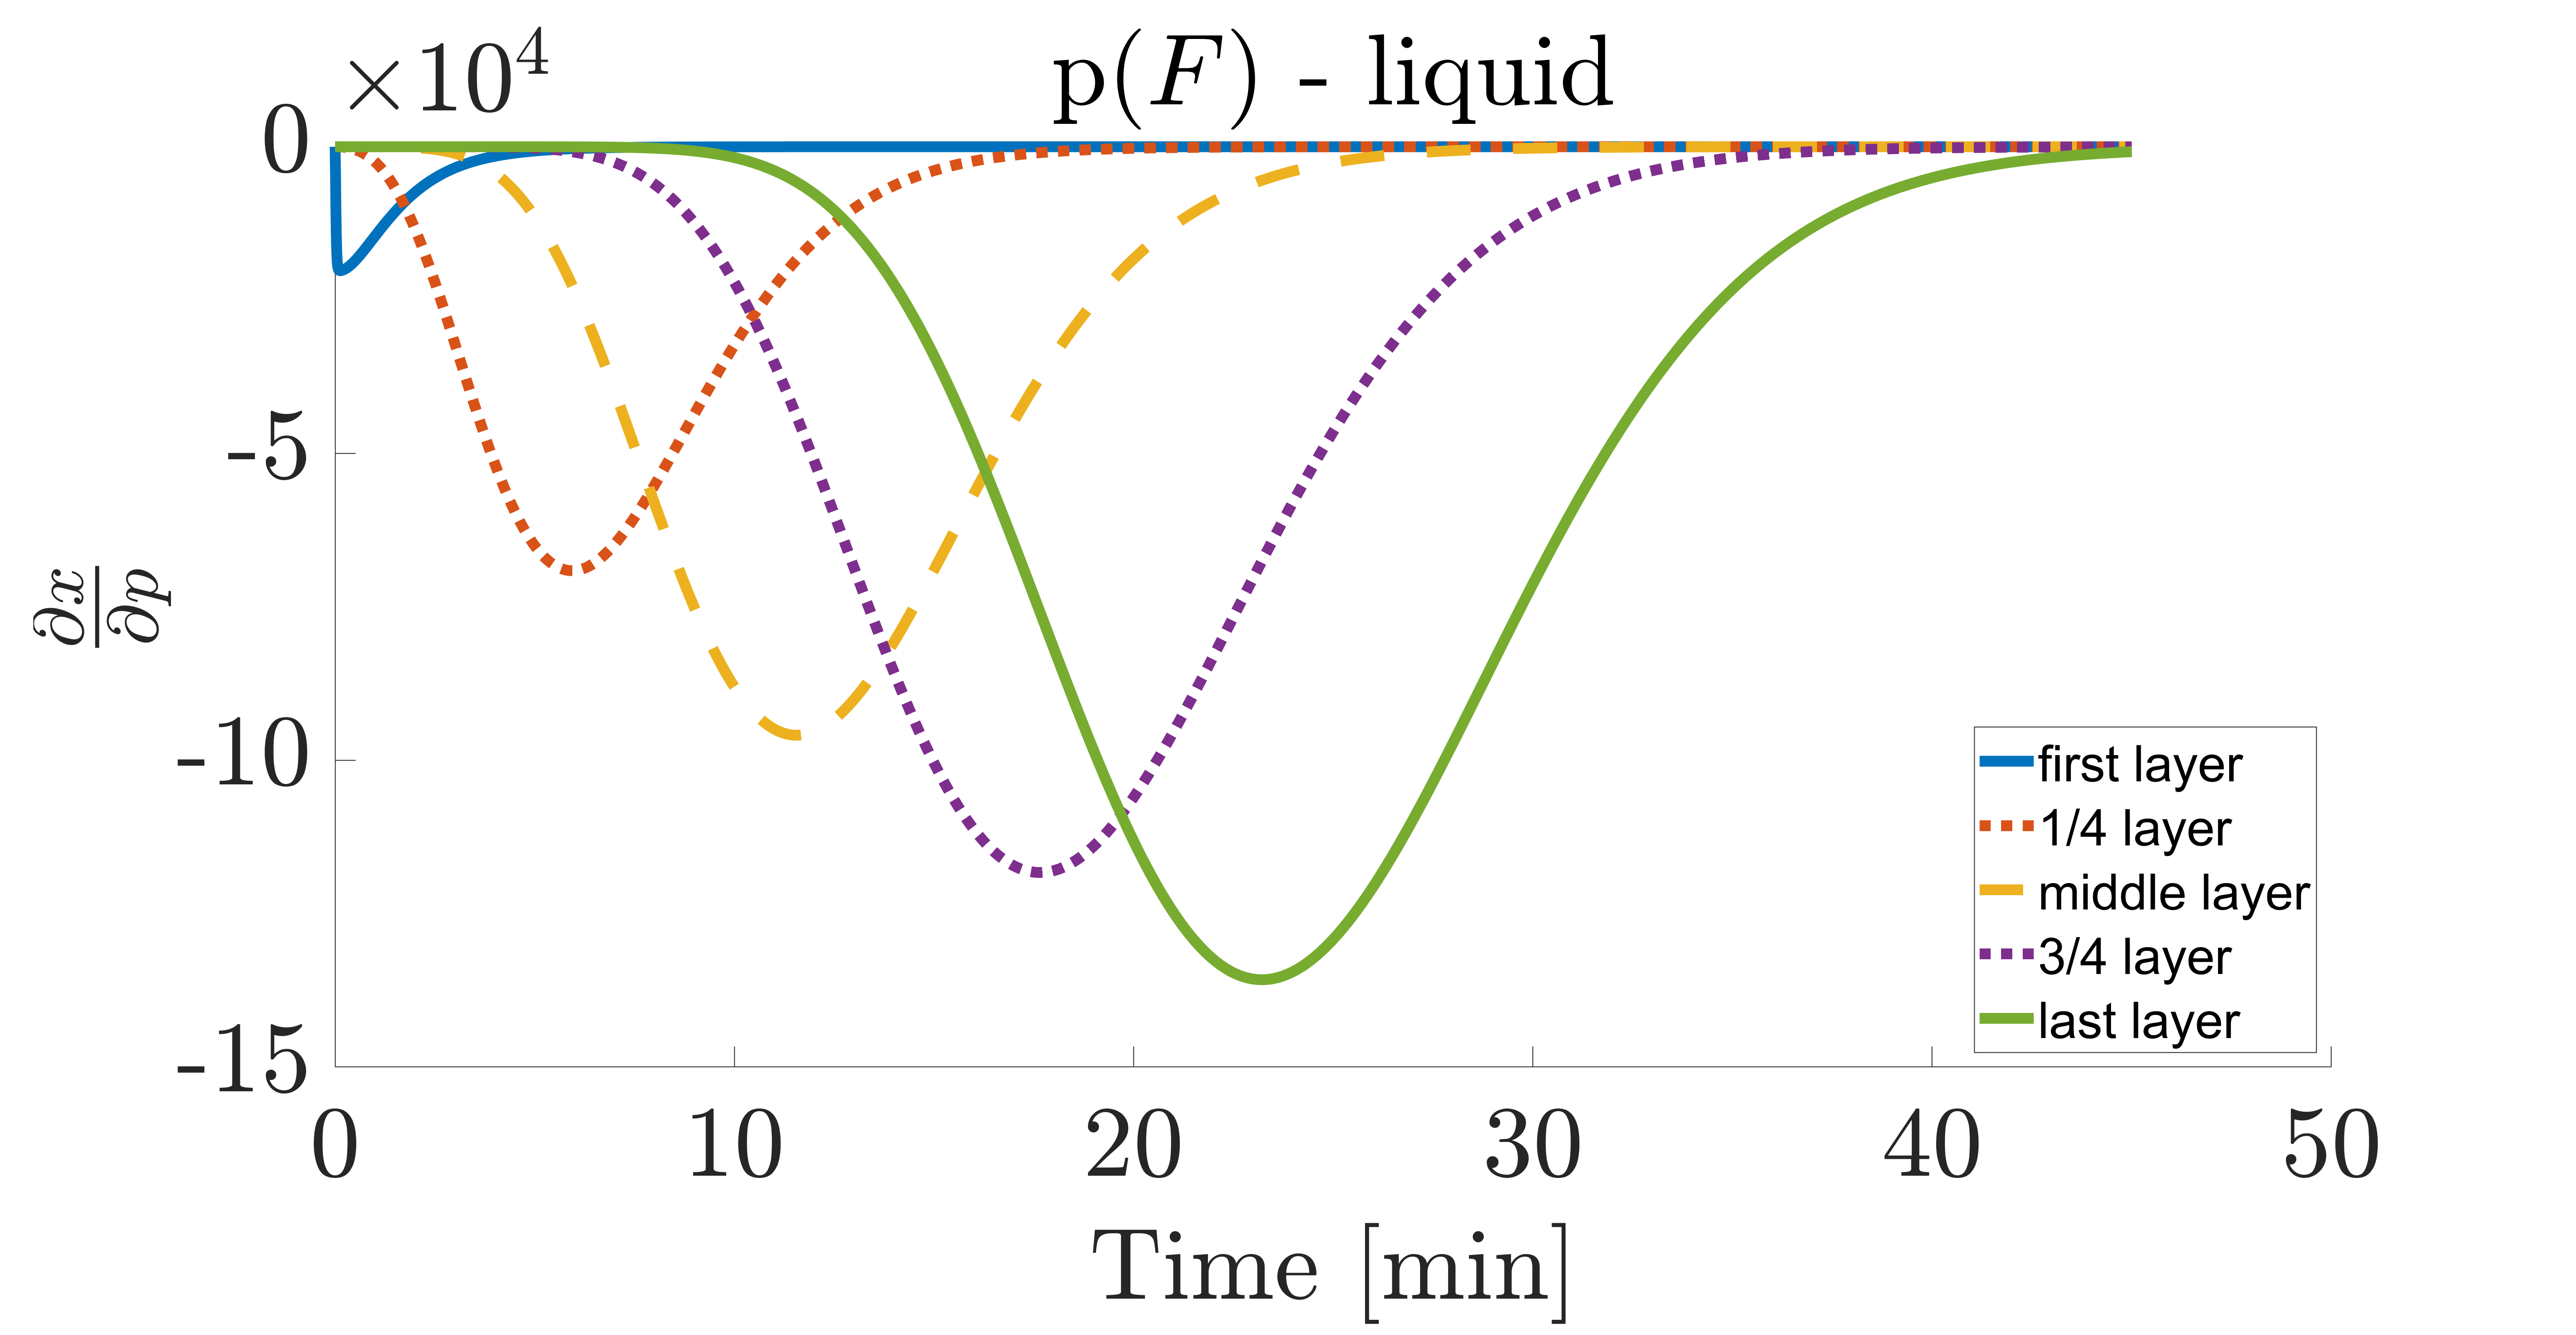
\includegraphics[width=3.7cm,height=2.0cm]{Figures/Sensitivity/Plots/2_SS_R_F.png}
		\column{.3\textwidth}
		\centering
		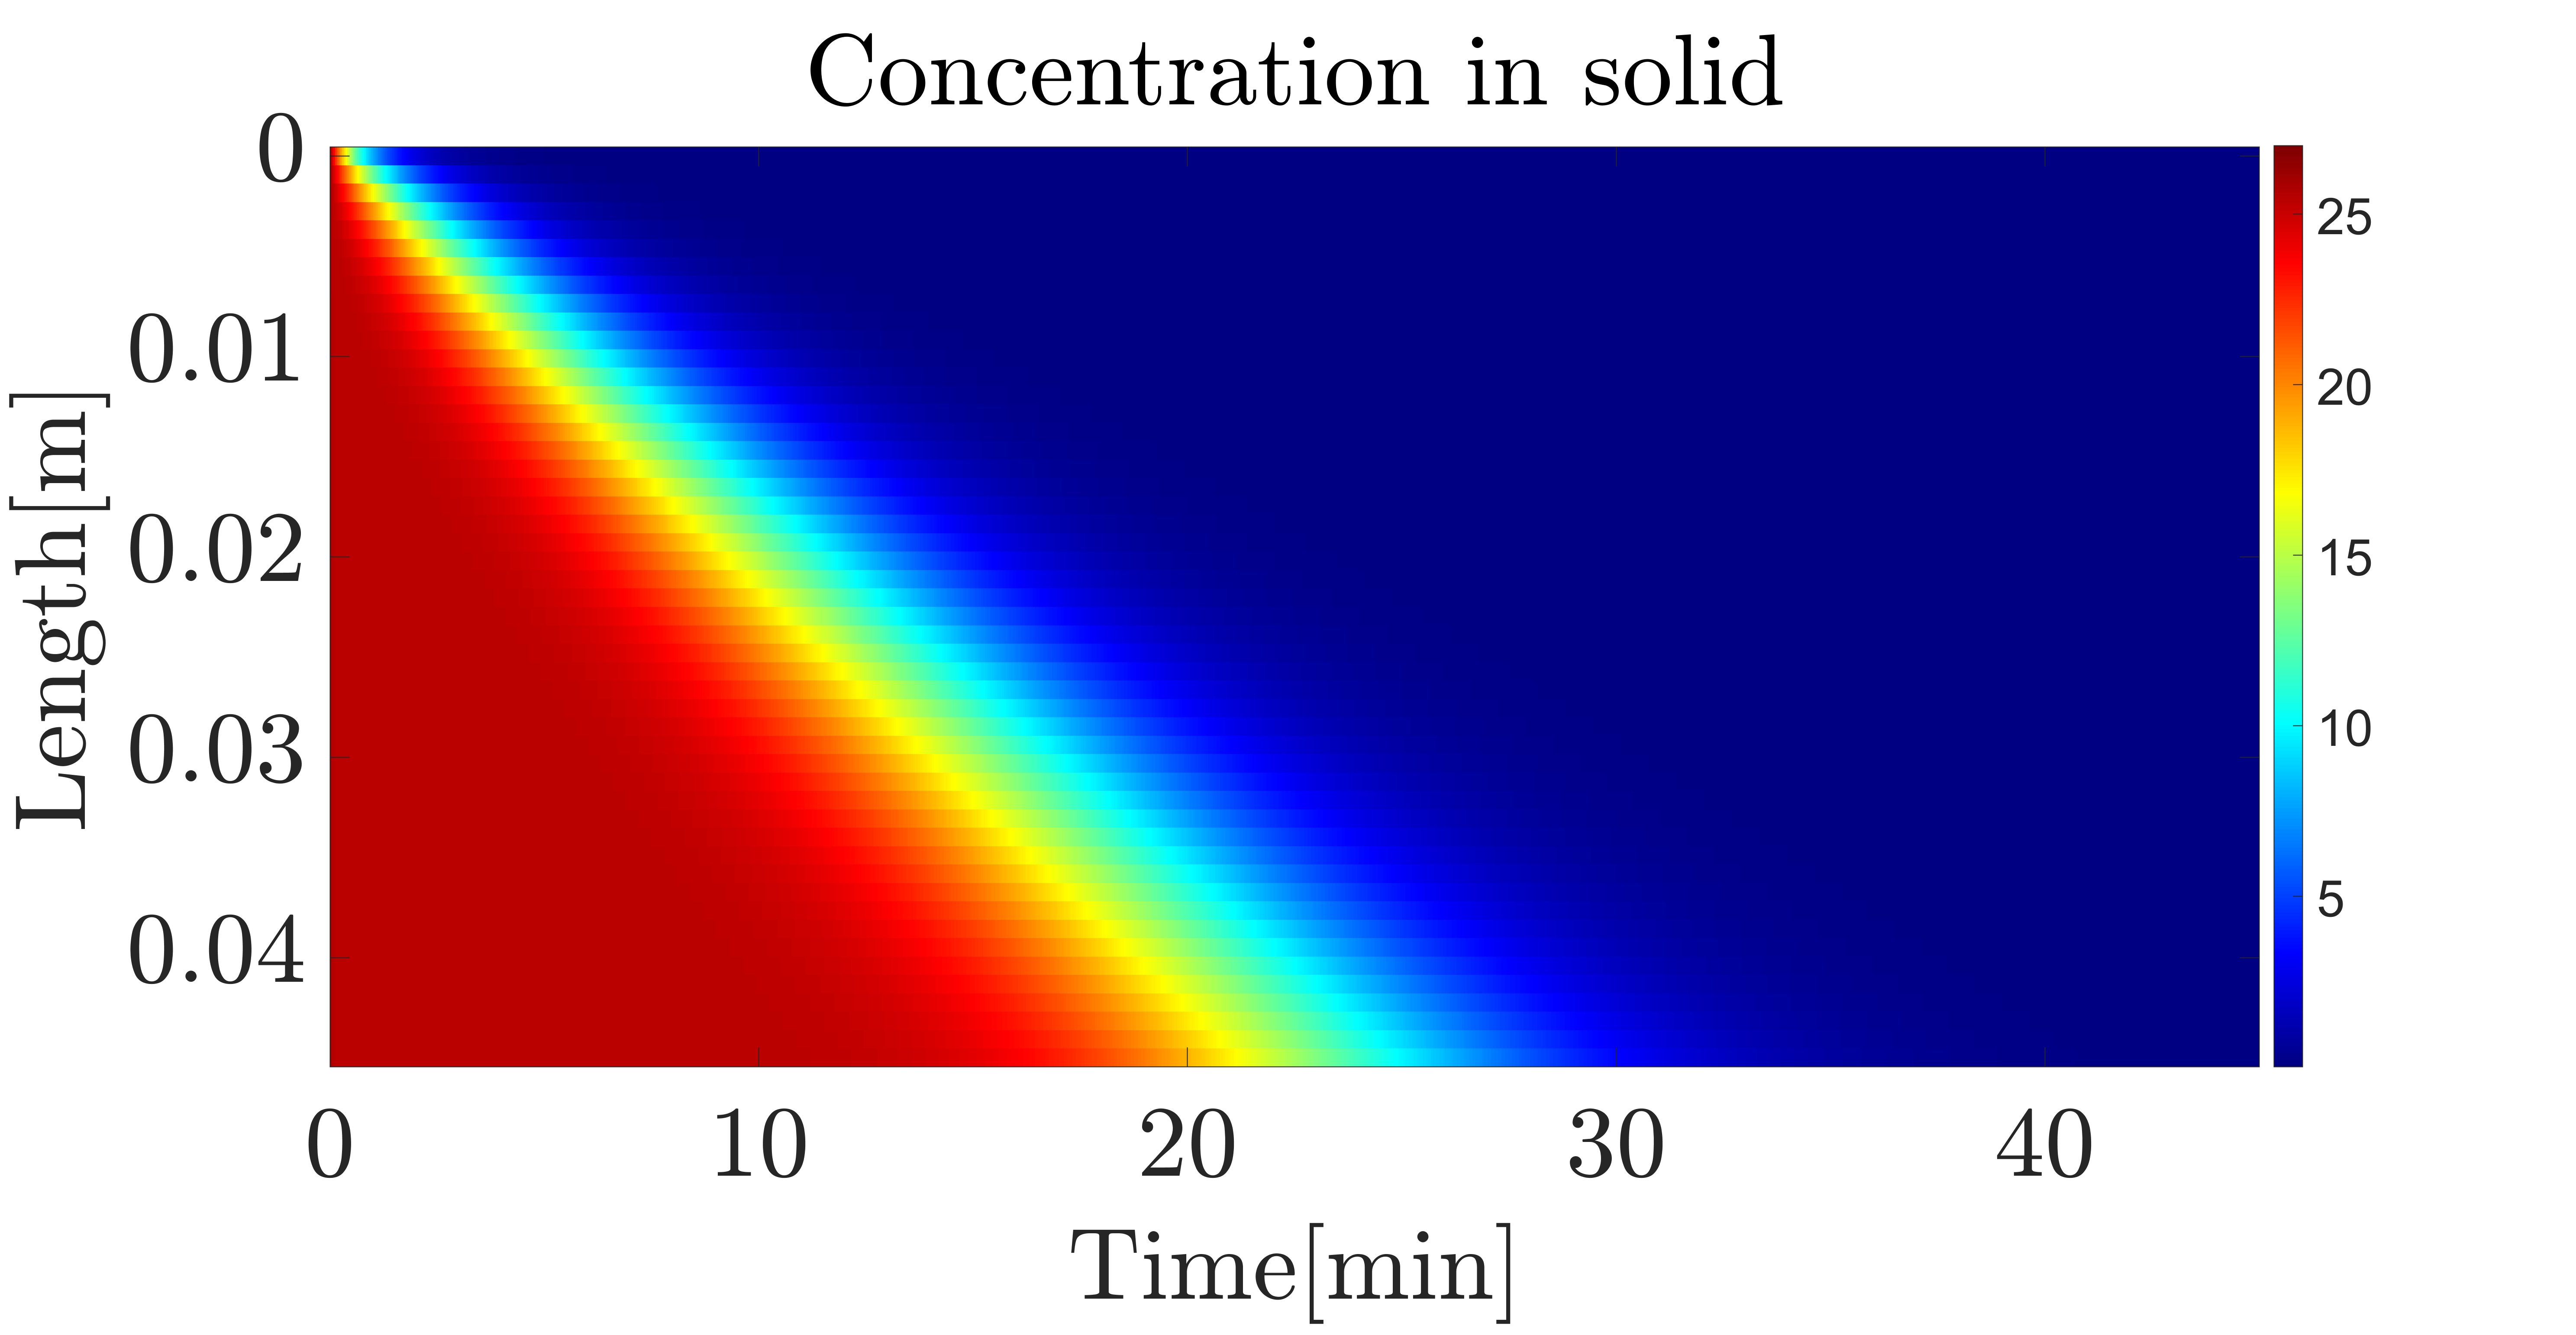
\includegraphics[width=3.7cm,height=2.05cm]{Figures/Sensitivity/ConcentrationSolid.png}\\
		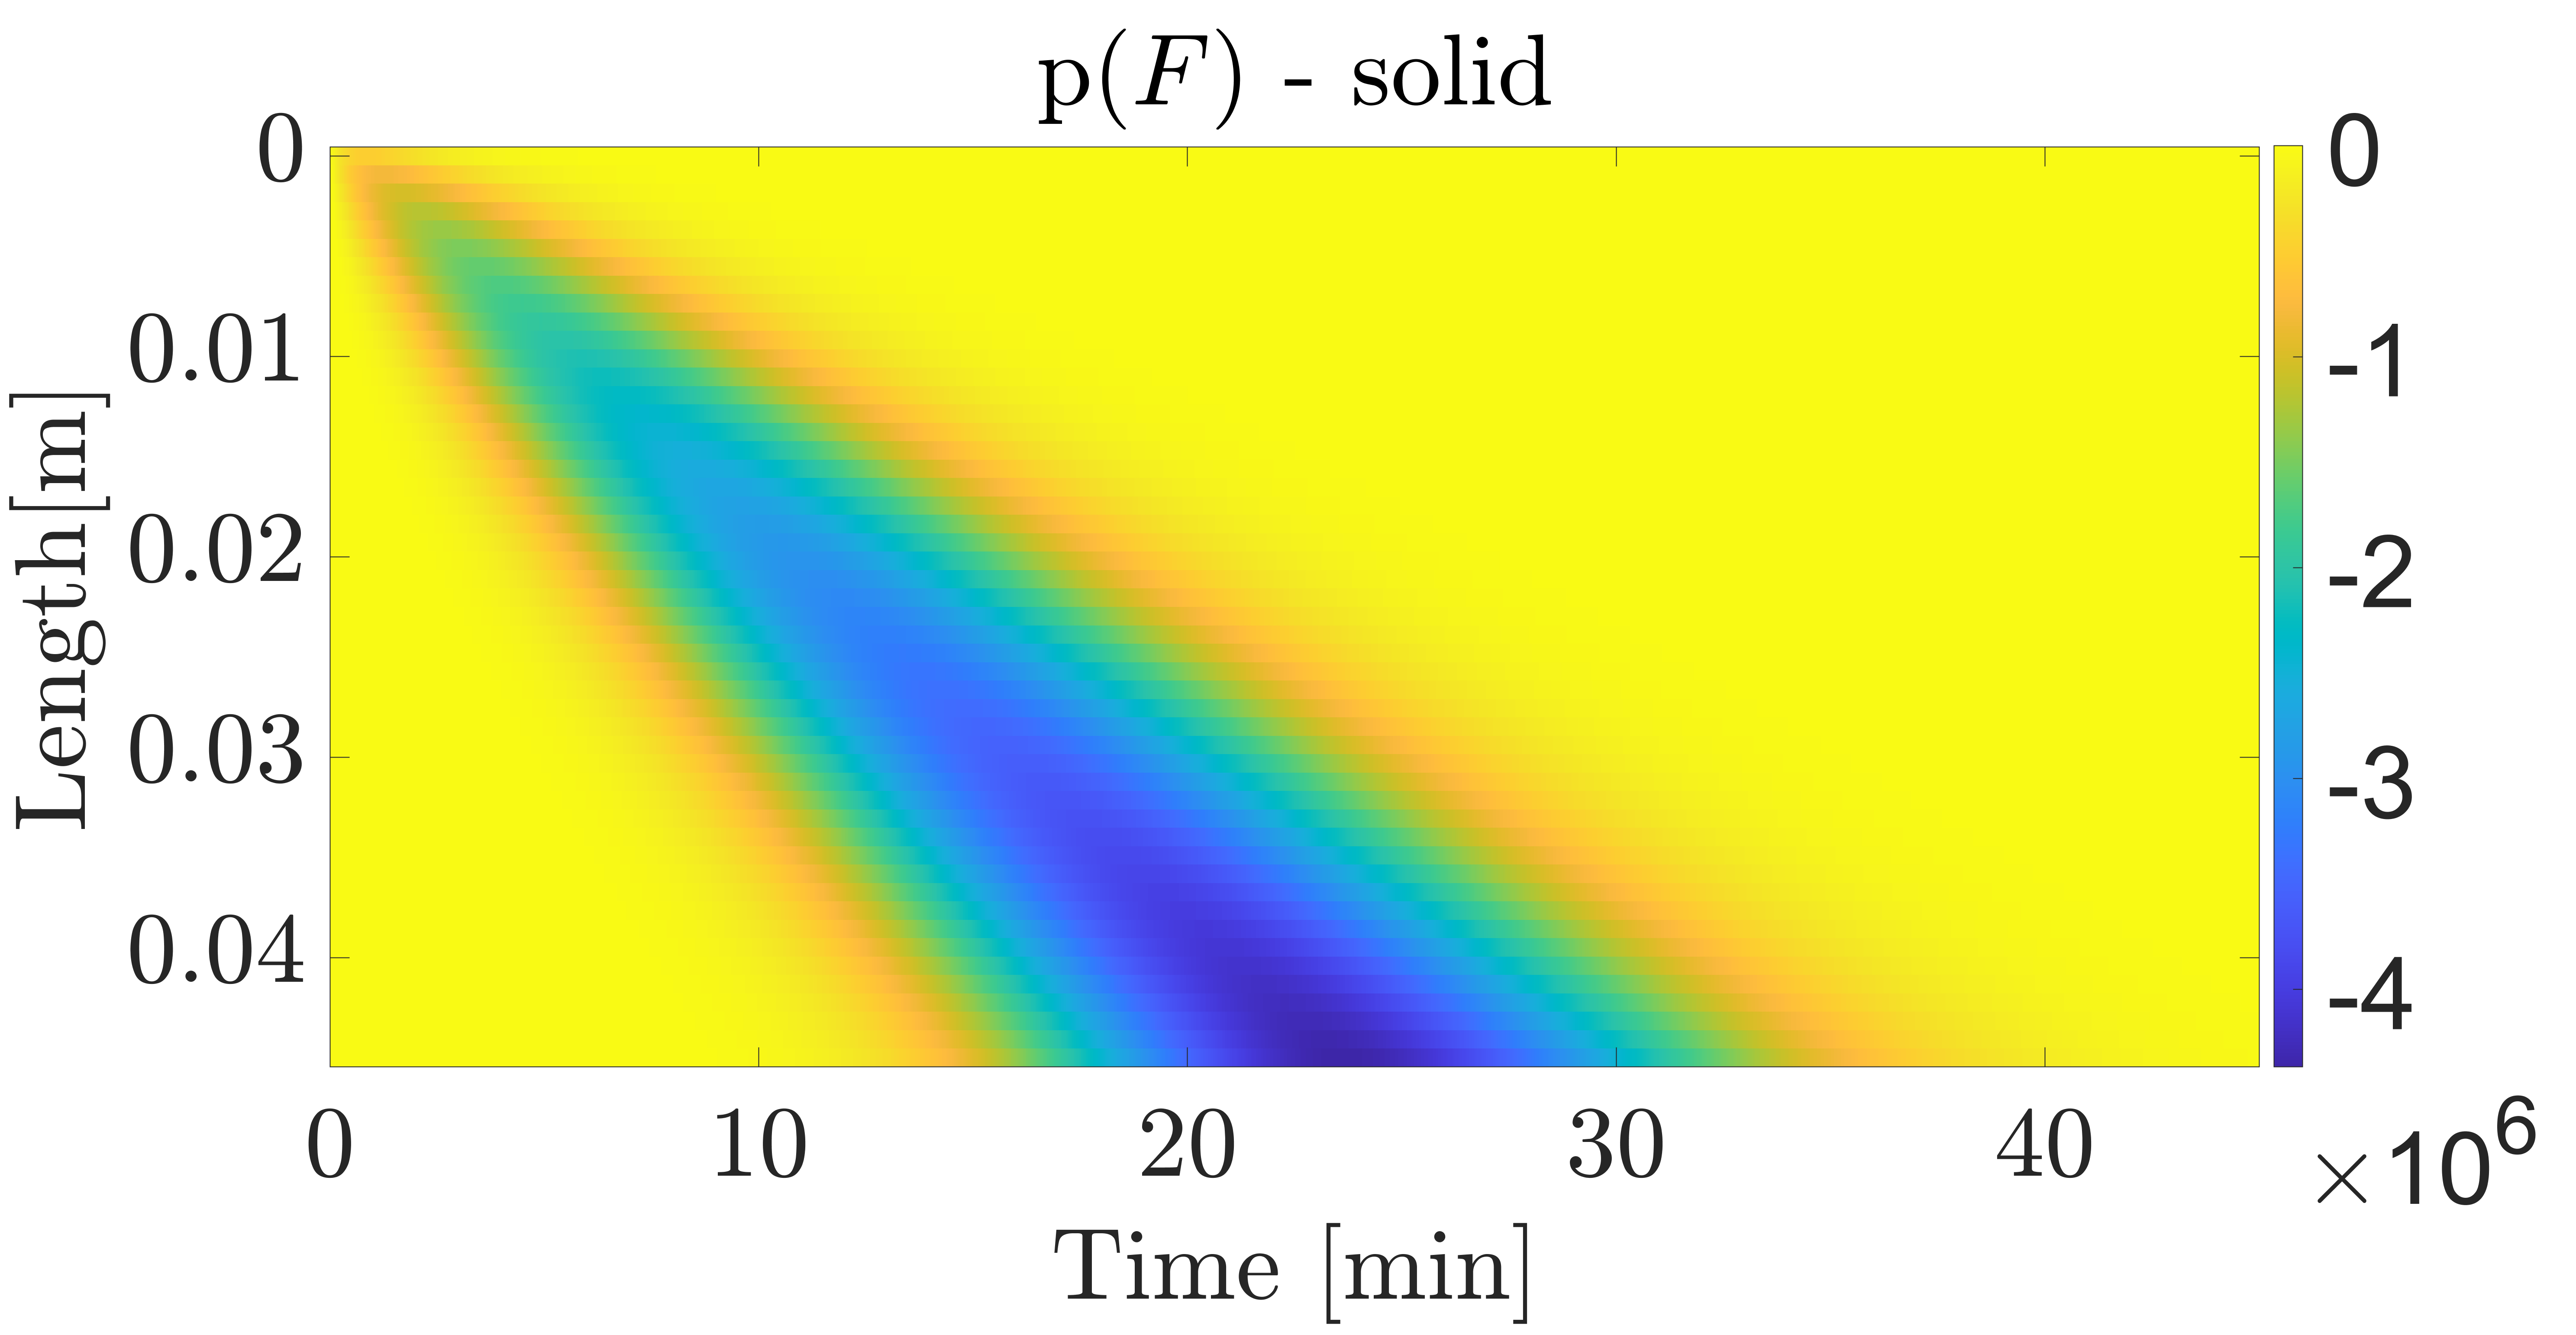
\includegraphics[width=3.7cm,height=2.0cm]{Figures/Sensitivity/Imagesc/3_SS_R_F.png}\\
		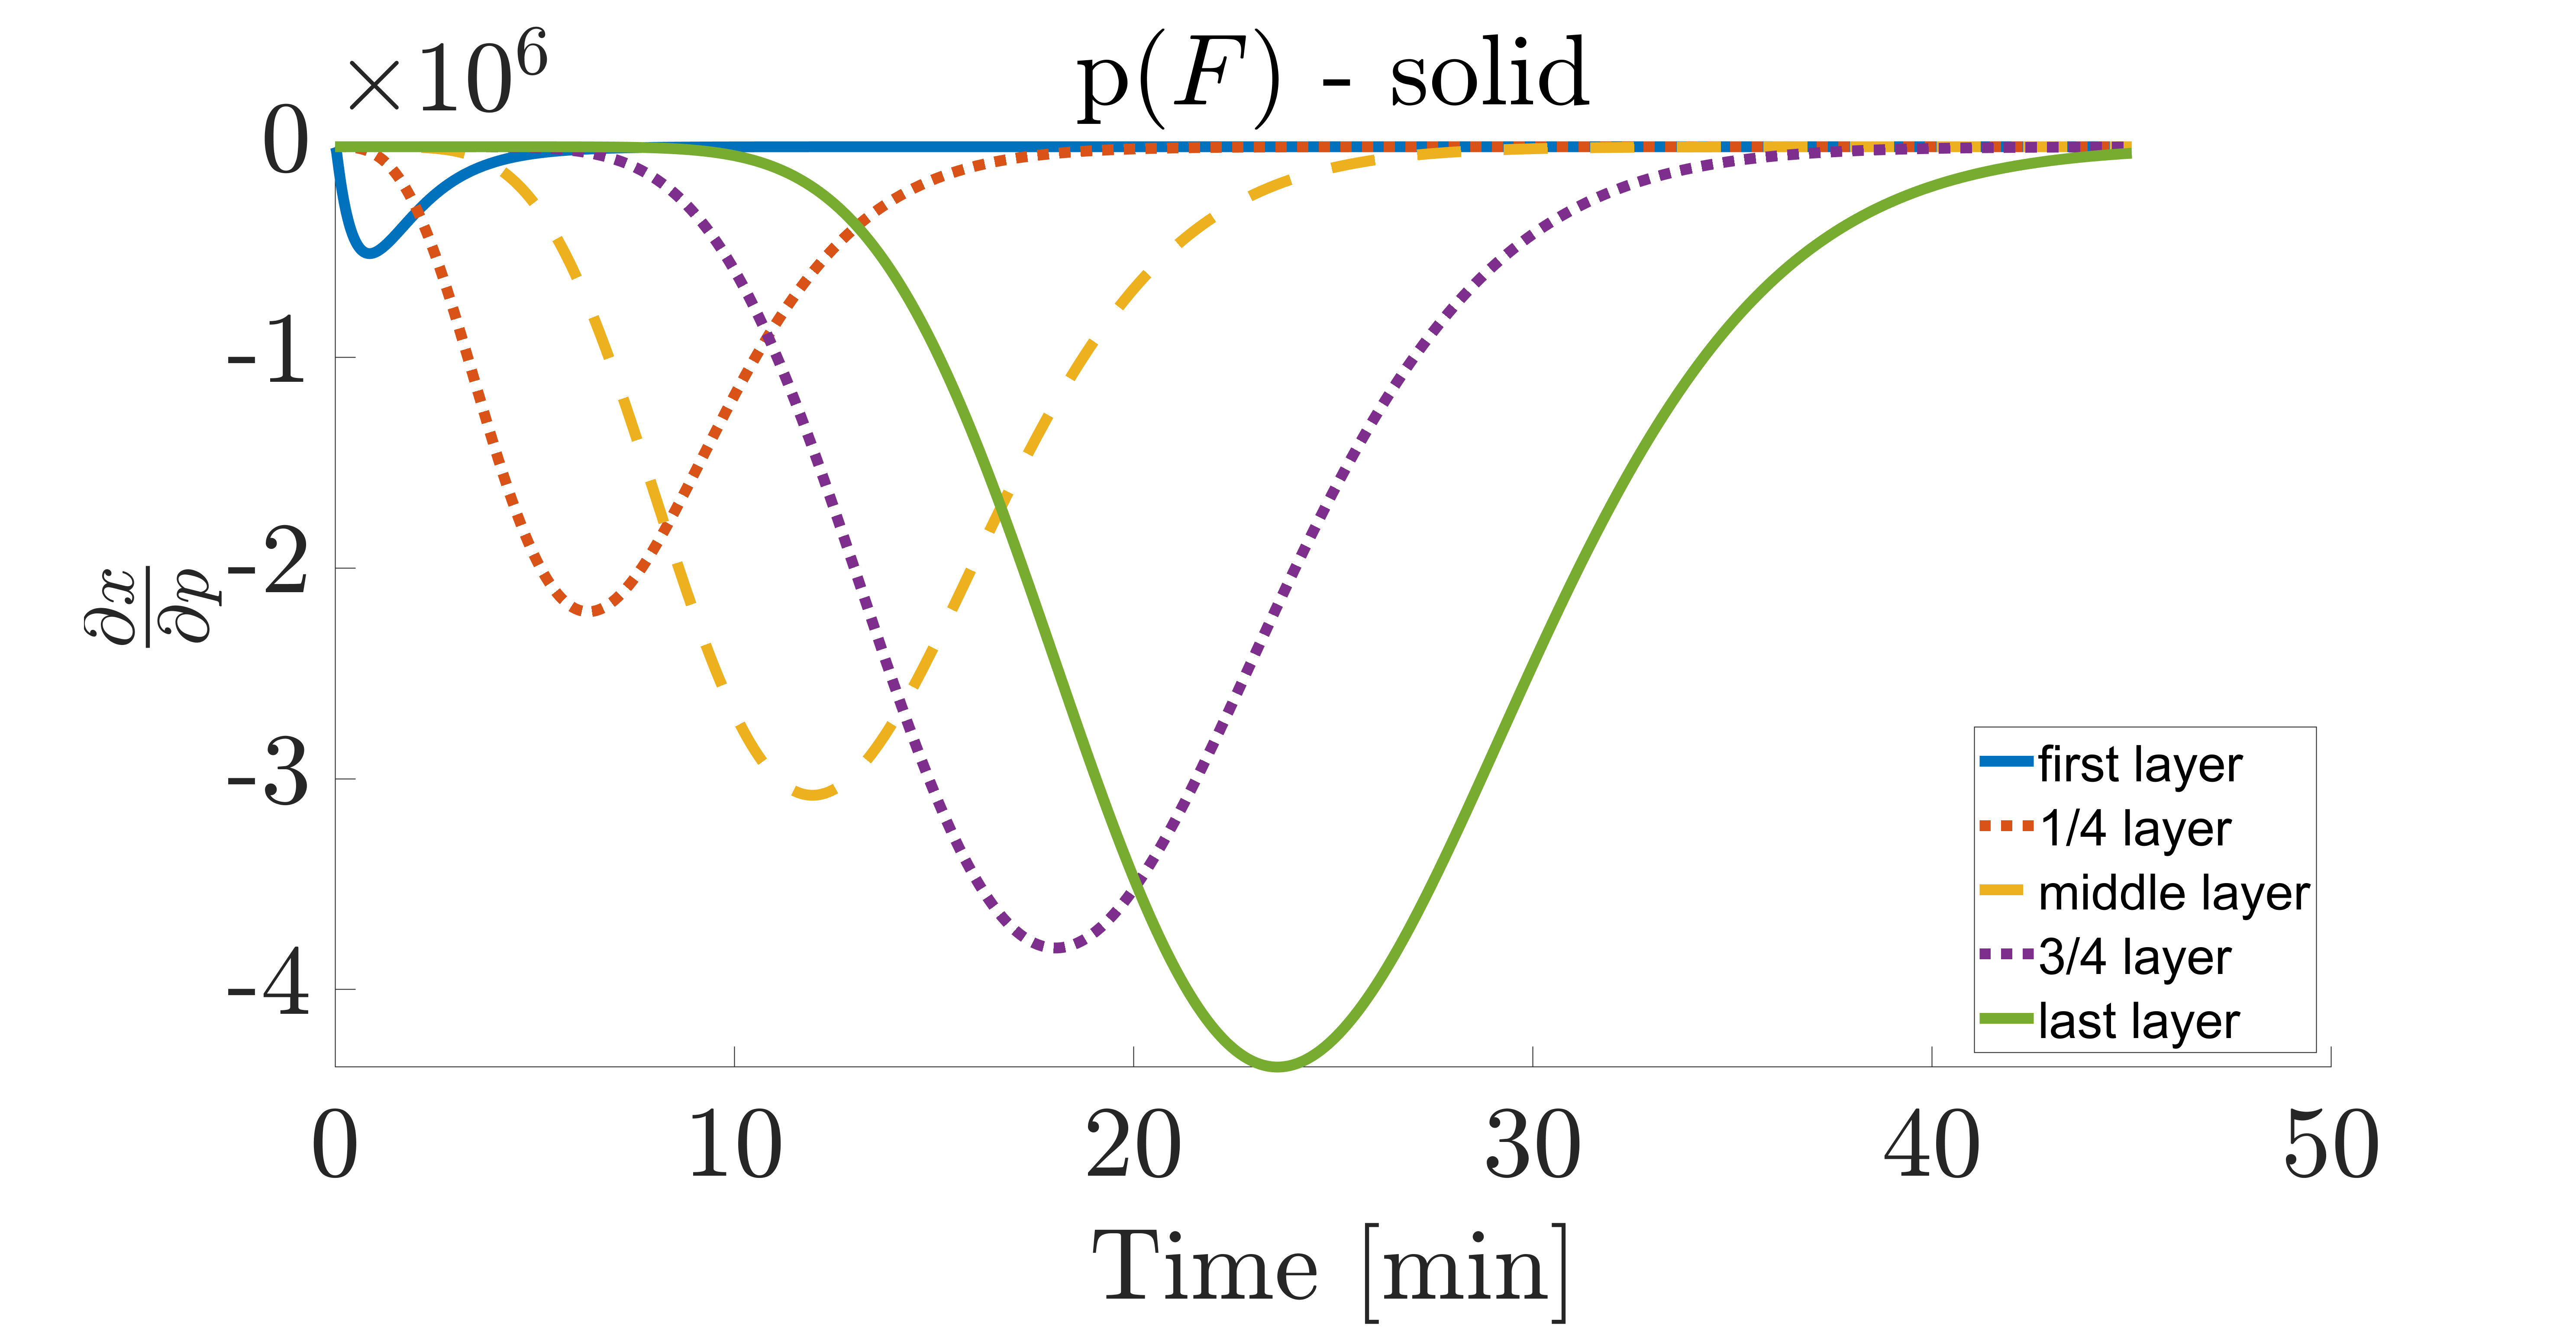
\includegraphics[width=3.7cm,height=2.0cm]{Figures/Sensitivity/Plots/3_SS_R_F.png}
		\column{.3\textwidth}
		\centering
		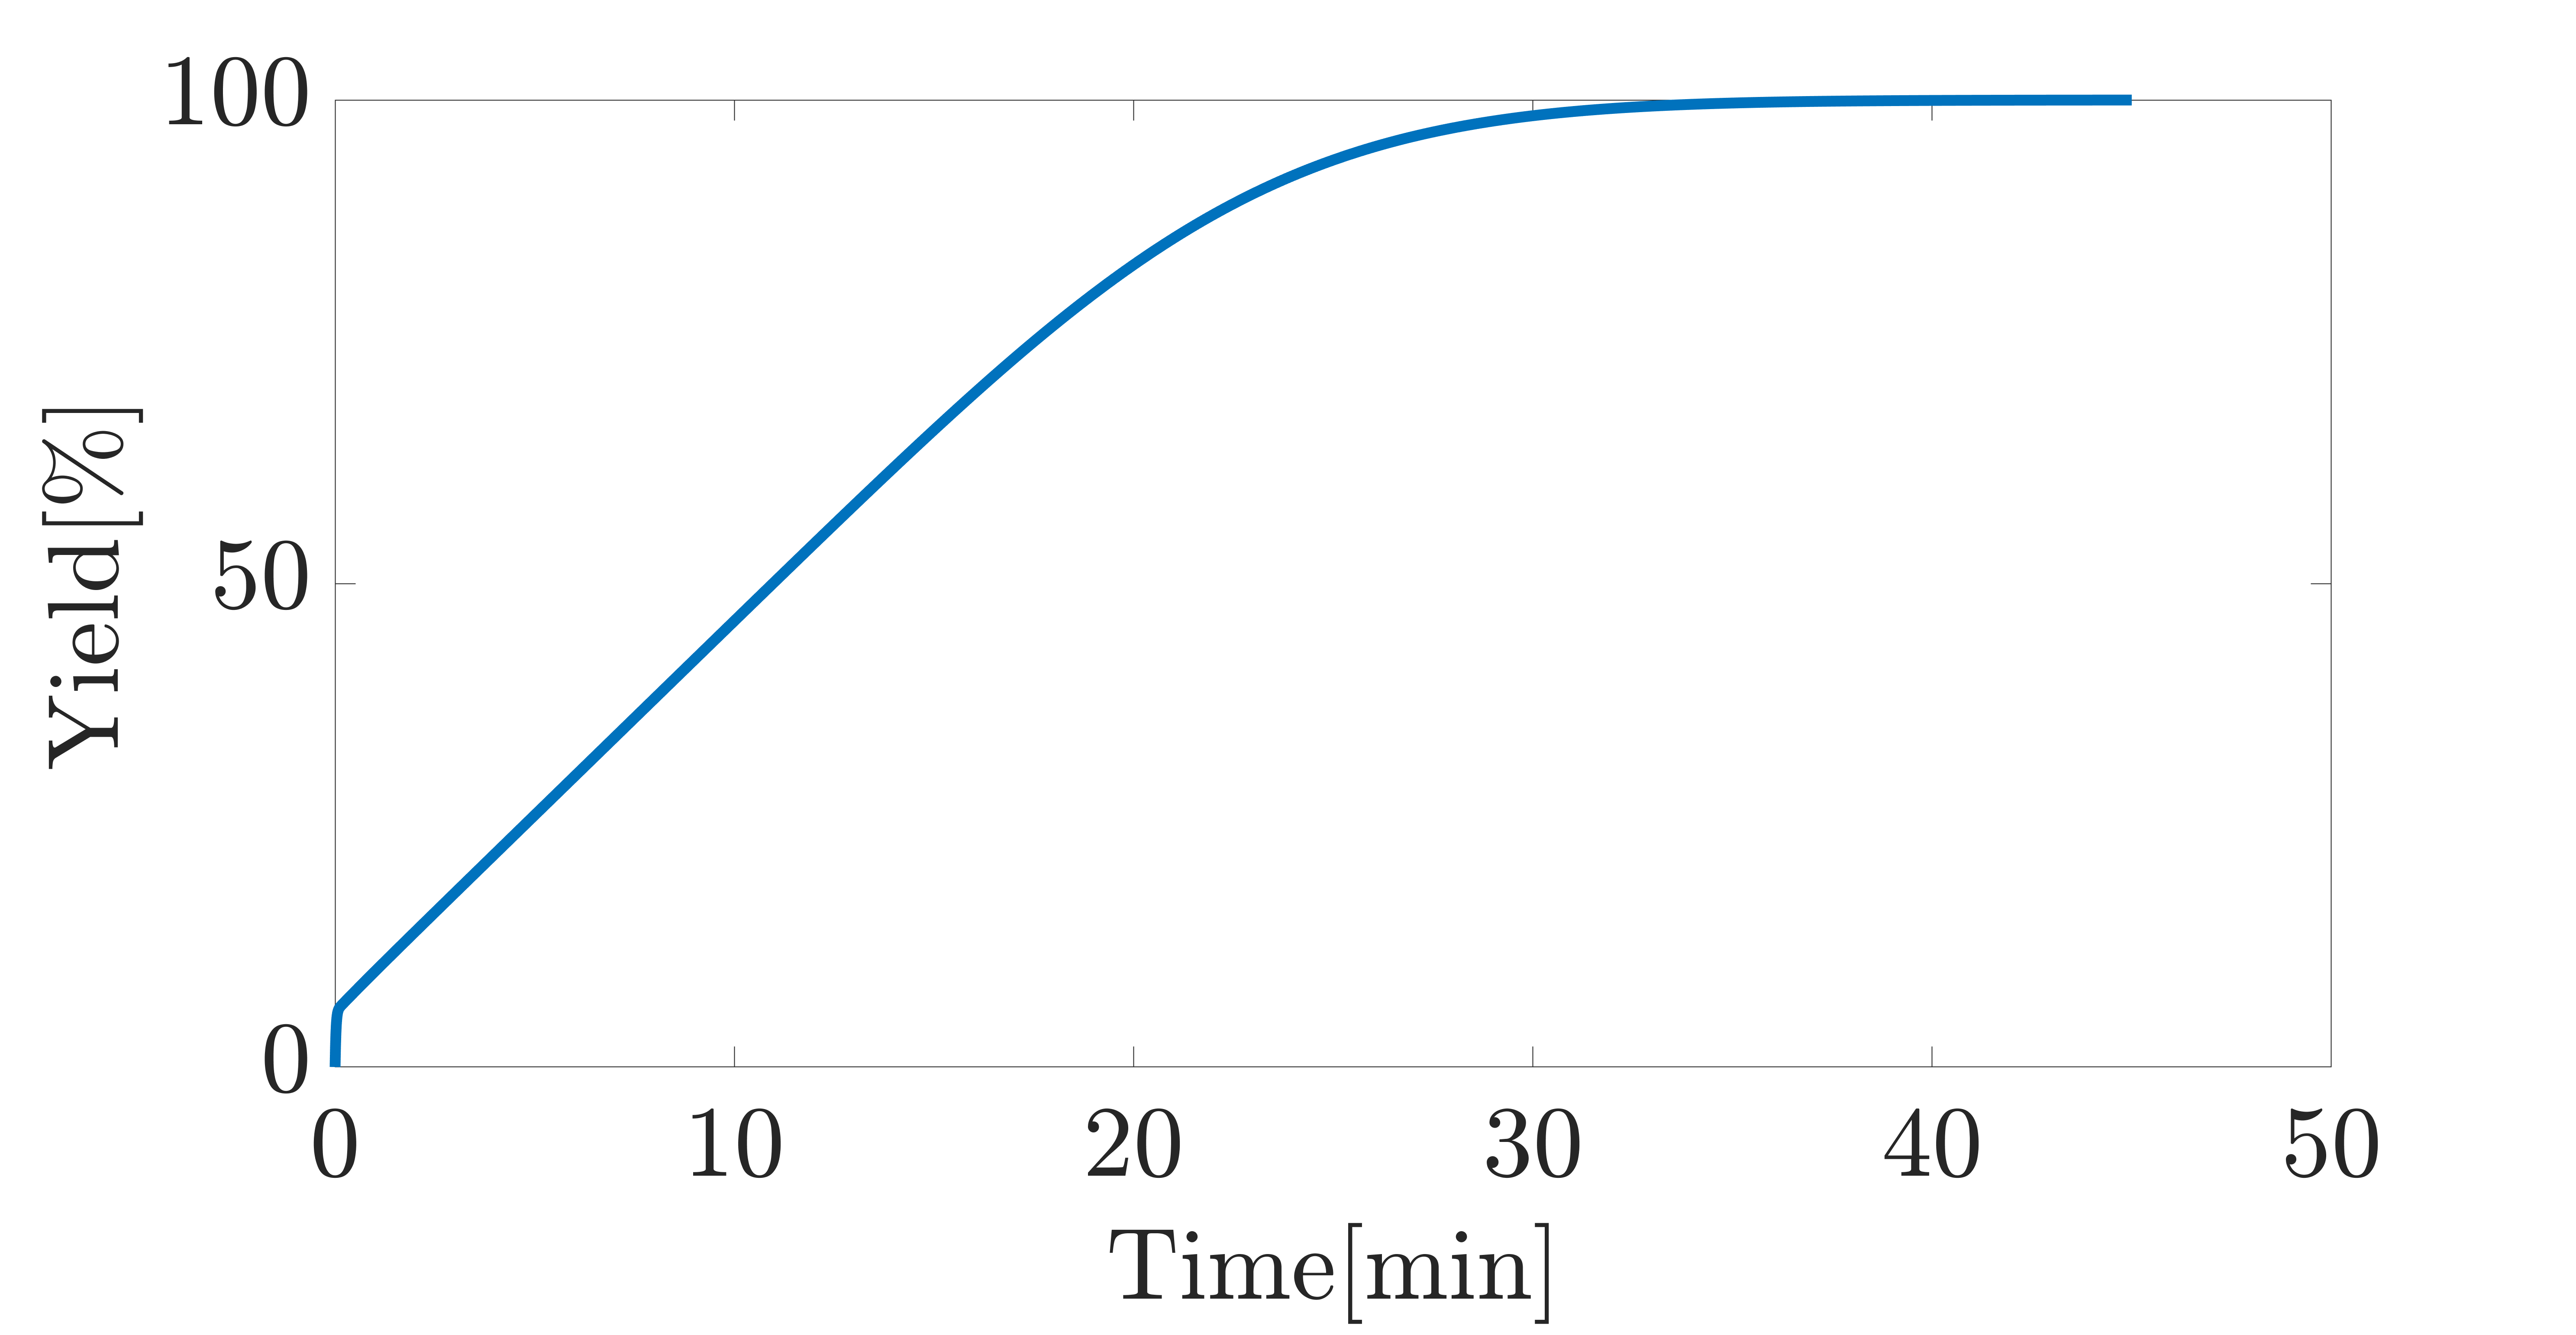
\includegraphics[width=3.7cm,height=2.0cm]{Figures/Sensitivity/Yield.png}\\
		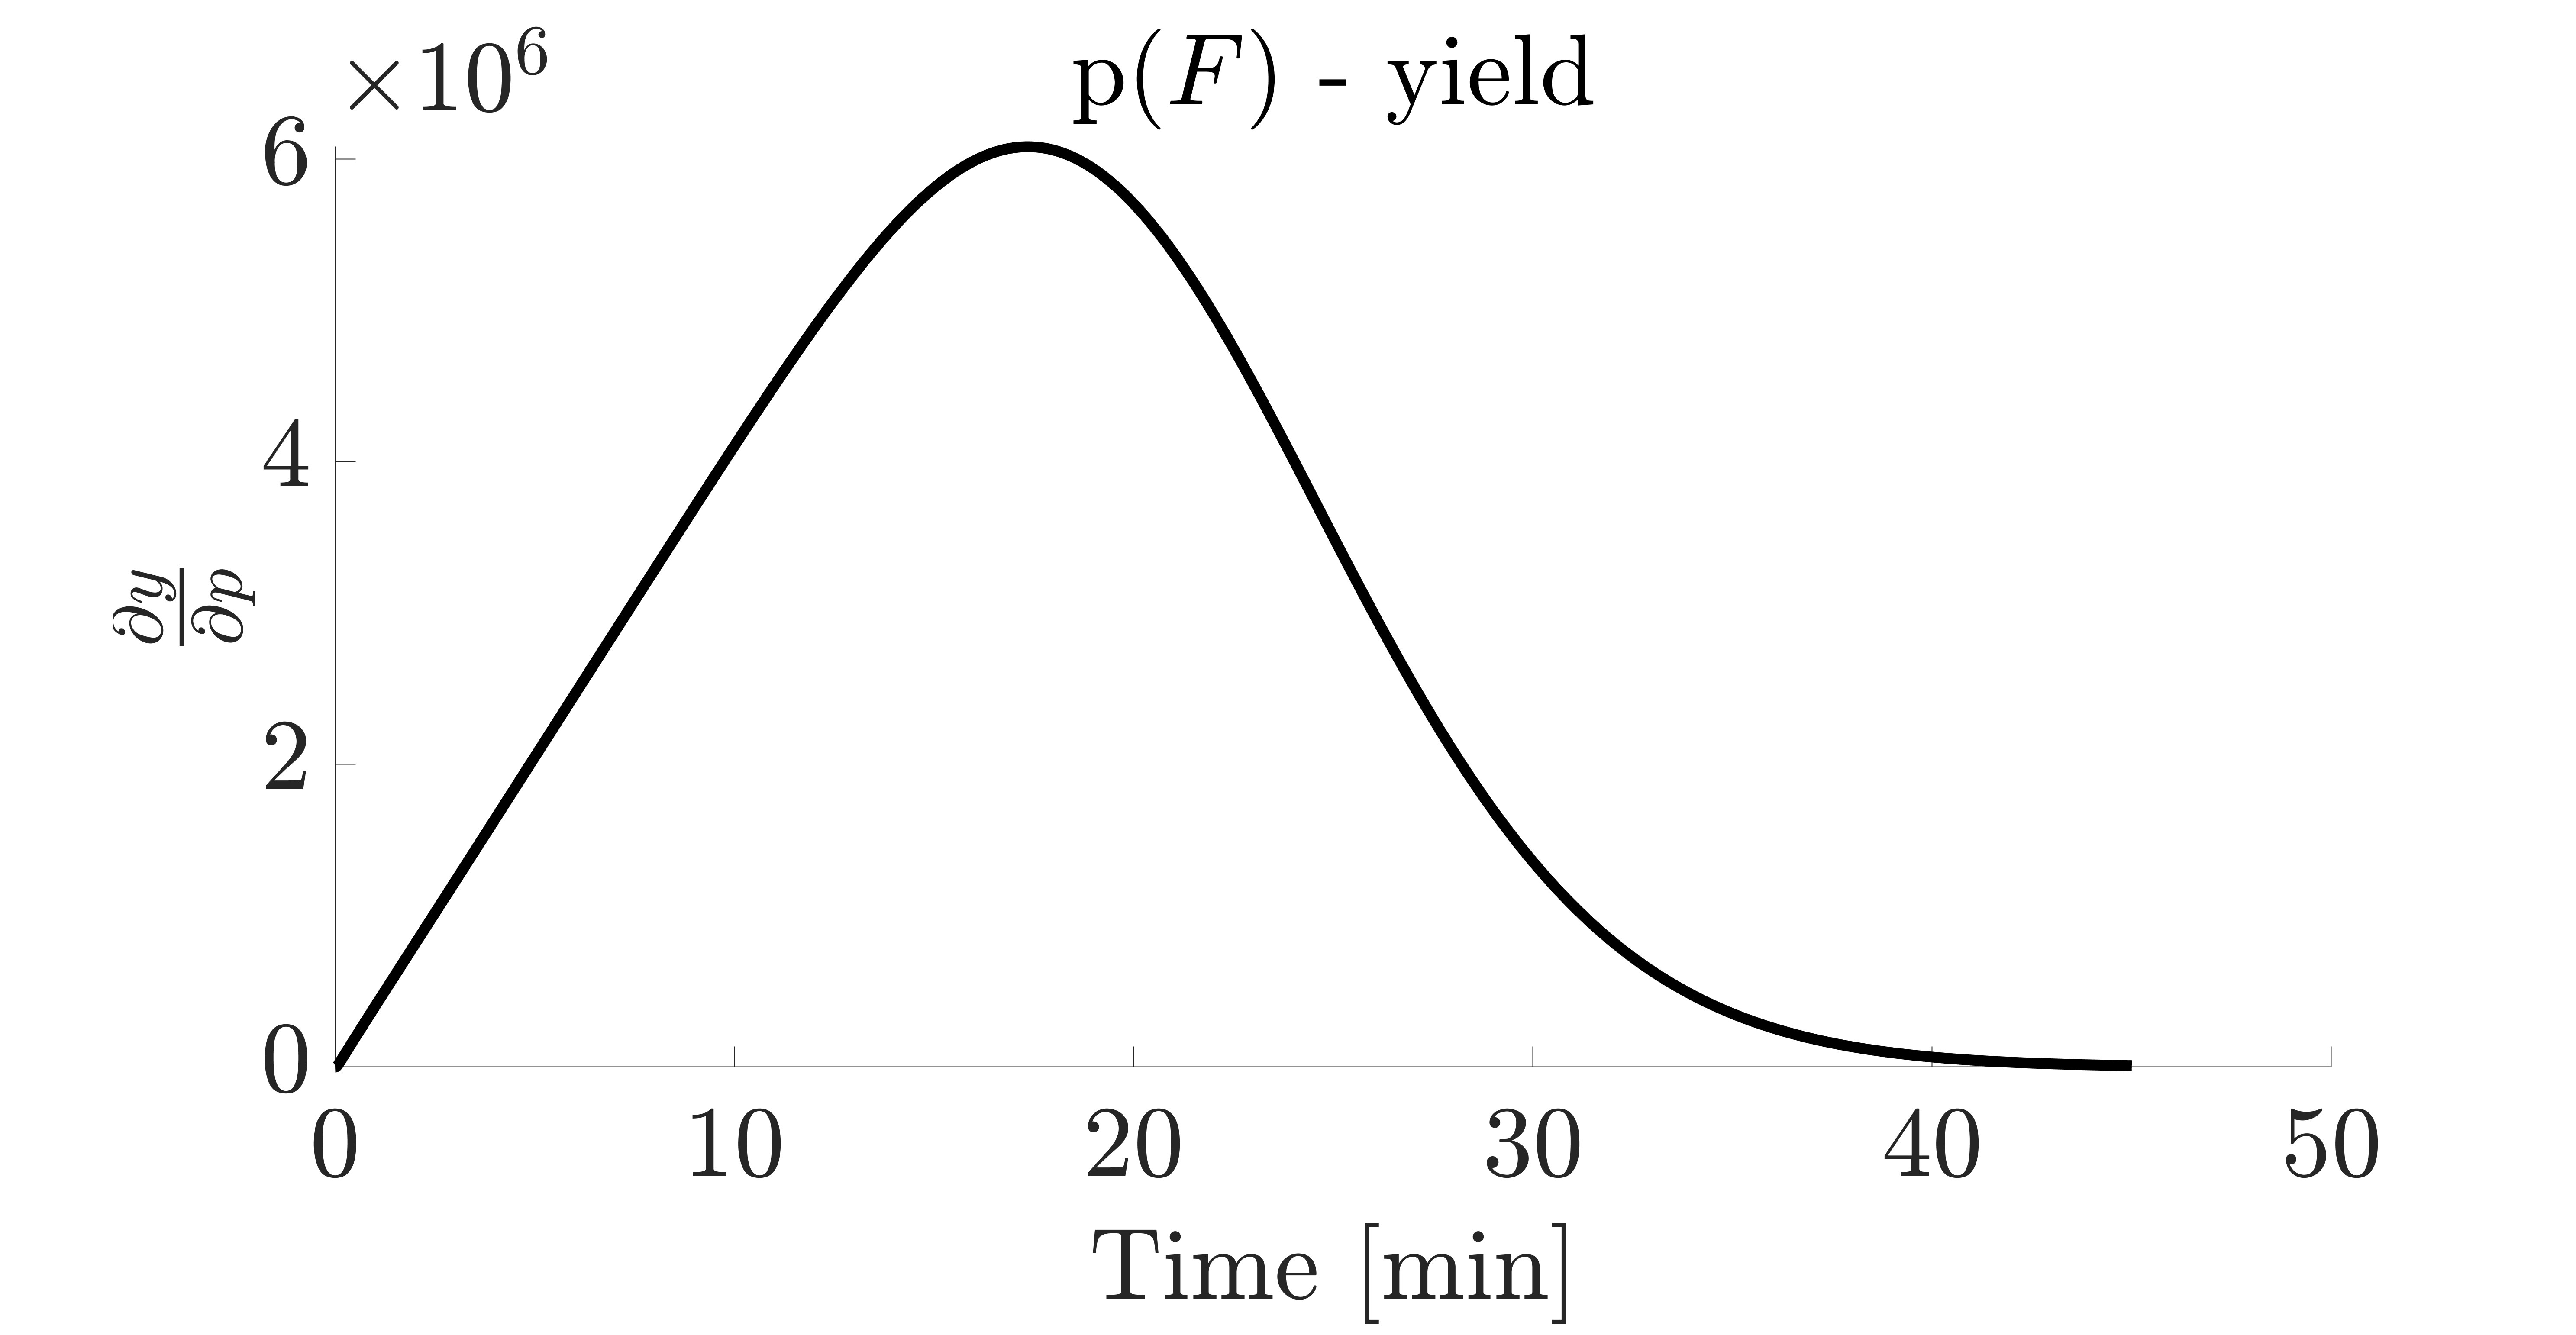
\includegraphics[width=3.7cm,height=2.0cm]{Figures/Sensitivity/Plots/1_SS_R_F.png}
	\end{columns}
\hrule
\footnotesize{[3] R.Vargas, Supercritical extraction of carqueja essential oil: experiments and modeling, Brazilian Journal of Chemical Engineering (2006) }
\end{frame}
	
\end{document}
